\documentclass[10pt,a4paper]{article}
\usepackage[margin=1.3cm]{geometry}
\usepackage[T1]{fontenc}
\usepackage{amsmath}
\usepackage{enumitem,booktabs,parskip,tikz}
\usetikzlibrary{arrows.meta,positioning}
\setlength{\parskip}{3pt}
\pagestyle{empty}

\begin{document}

\begin{center}
  {\LARGE\bfseries Claim to Fame --- Team Oasis}\\[2pt]
  {\small Technical Report \;·\; QuantCo Agentic Hackathon, Munich \;·\; August 22--23, 2026}
\end{center}
\vspace{-2pt}\hrule\vspace{5pt}

\textbf{Approach.} We treated the game as an estimation problem wrapped in game theory,
played \emph{against the field}: a fair charge is paid by every reviewer (rejecting it
costs them $1.5a$), overcharging is free, and accepting is only correct when
$P(\mathrm{fair}) > 2/3$ --- so the policy layer follows from the payoff rules, not from
intuition. Because every team's transactions are public, we mined $250$k+ of them into
proven price intervals: the field's mistakes are measurable, and its review errors are
our income. Every mechanism was backtested against this truth base before going live.

\section*{Pipeline per round (12-min cadence, $\sim$10--25\,s runtime)}
\vspace{-4pt}
\begin{center}
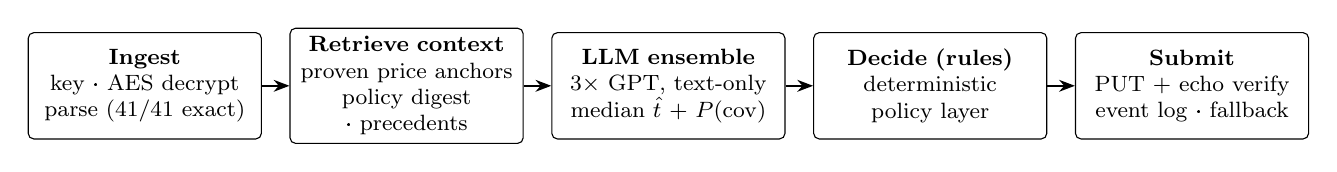
\begin{tikzpicture}[
  box/.style={draw, rounded corners=2pt, align=center, font=\footnotesize,
              minimum height=1.35cm, text width=2.75cm, inner sep=3pt},
  arr/.style={-{Stealth[length=2mm]}, thick}]
  \node[box] (a) {\textbf{Ingest}\\ key · AES decrypt\\ parse (41/41 exact)};
  \node[box, right=3.5mm of a] (b) {\textbf{Retrieve context}\\ proven price anchors\\ policy digest · precedents};
  \node[box, right=3.5mm of b] (c) {\textbf{LLM ensemble}\\ $3\times$ GPT, text-only\\ median $\hat t$ + $P(\mathrm{cov})$};
  \node[box, right=3.5mm of c] (d) {\textbf{Decide (rules)}\\ deterministic\\ policy layer};
  \node[box, right=3.5mm of d] (e) {\textbf{Submit}\\ PUT + echo verify\\ event log · fallback};
  \draw[arr] (a) -- (b); \draw[arr] (b) -- (c);
  \draw[arr] (c) -- (d); \draw[arr] (d) -- (e);
\end{tikzpicture}
\end{center}

\section*{The decision rules (the entire policy layer)}
\vspace{-4pt}
\begin{itemize}[leftmargin=1.3em, itemsep=1pt]
  \item \textbf{Issuer:} $a = 0.9\,\hat t$, never lowered under uncertainty --- a fair
        charge is paid by all 16 reviewers either way, and overcharging carries no
        penalty. Provably worthless items are still charged (zero-floor): rejection
        costs nothing, careless acceptors pay.
  \item \textbf{Reviewer:} $b = m \cdot \hat t$ with value-tiered $m = 0.9/1.0/1.0$,
        a global cap of $800$, and downward clamps to proven fraud ceilings of similar
        items (anchor evidence).
  \item \textbf{Coverage gate:} ensemble $P(\mathrm{cov}) < 1/3$ $\Rightarrow$ treat as
        excluded ($b=0$, charge floored \emph{up}); $P(\mathrm{cov}) < 2/3$
        $\Rightarrow$ keep the charge but accept nothing.
  \item \textbf{Operations:} every knob lives in \texttt{policy.json}, hot-reloaded
        before each round --- five backtested policy changes went live within one hour.
\end{itemize}

\section*{Evidence base}
\vspace{-4pt}
\begin{center}
\begin{tabular}{@{}p{9.2cm}l@{}}
\toprule
Reconstruction of the official score matrix (1{,}700 cells) & error $= 0.0000$\\
Public transactions $\rightarrow$ proven $t$-intervals & $250$k+ $\rightarrow$ $1{,}161$\\
Price anchors, leave-one-game-out backtest & income $+17\,\%$, cost $-14\,\%$\\
Acceptance cap $450 \rightarrow 800$ (561 real rejected charges) & $+12.8$k; live twin-case A/B: penalties $-72\,\%$\\
\bottomrule
\end{tabular}
\end{center}

\section*{Final phase (3$\times$ scoring) --- and the finale}
\vspace{-4pt}
\begin{center}
\begin{tabular}{@{}lrrl@{}}
\toprule
Round & Result & Rank & \\
\midrule
Game 88  & $+134{,}439$\,€ & 3/17 & highest issuer income of all teams\\
Game 92  & $+46{,}477$\,€  & 2/17 & twin-case A/B confirms cap thesis\\
Game 96  & $+64{,}814$\,€  & \textbf{1/17} & round win, $+23$k margin\\
Game 99  & $+39{,}678$\,€  & 3/17 & \\
\textbf{Game 100 (finale)} & \textbf{+134{,}957\,€} & \textbf{1/17} & \textbf{won the last game --- our biggest result, $+32$k margin}\\
\midrule
\multicolumn{4}{@{}p{16.8cm}@{}}{\textbf{13 of 14 final rounds positive, $+575.5$k} · \#1 issuer income
of all 17 teams over that stretch · comeback from $-915$k to $-357$k, final rank 9/17 (up from 13).}\\
\bottomrule
\end{tabular}
\end{center}

\section*{Takeaways}
\vspace{-4pt}
\begin{itemize}[leftmargin=1.3em, itemsep=0pt]
  \item \textbf{Game theory before ML:} the payoff asymmetries define the optimal policy; better estimation only pays after that.
  \item \textbf{Calibration beats capacity:} more context and stronger models both made estimates bolder, not better --- measured, twice.
  \item \textbf{It is a market, not a quiz:} public data $\neq$ public alpha --- the edge came from processing the field's own traces
        with strict validation discipline.
\end{itemize}

\vspace{2pt}\hrule\vspace{3pt}
{\footnotesize\emph{Among the things we tried and measured along the way:} hybrid RAG over
policy clauses (cannot predict $t$ alone, kept as precedent memory for recycled cases) ·
a benchmark across the GPT model family (median of three small text-only models won) ·
probabilistic coverage masks (ported corrected: $p$ gates only acceptance, never the
charge) · an anchor floor on acceptance limits (removed after a cross-trade collision) ·
a measured fraud-tolerance curve of the field ($\sim$17--23\,\%, nearly height-independent).}

\end{document}
